\documentclass[11pt,a4paper]{article}

\usepackage[utf8]{inputenc}
\usepackage[T1]{fontenc}
\usepackage[french]{babel}
\usepackage{lmodern}
\usepackage{amsmath,amssymb,amsthm,amsfonts,mathtools,bm}
\usepackage[margin=2.4cm]{geometry}
\usepackage{xcolor}
\usepackage{hyperref}
\hypersetup{colorlinks=true,linkcolor=blue!60!black,urlcolor=blue!60!black,
  citecolor=blue!60!black}
\usepackage{graphicx}
\usepackage{booktabs}
\usepackage{caption}
\usepackage{subcaption}
\usepackage{enumitem}
\usepackage{fancyhdr}
\usepackage{authblk}

\renewcommand{\baselinestretch}{1.10}

\newcommand{\R}{\mathbb{R}}
\newcommand{\Ta}{T_a}
\newcommand{\We}{\mathit{We}}
\newcommand{\Rey}{\mathit{Re}}
\newcommand{\projname}{\textsc{TaylorCouetteML}}

% Nouvelles architectures (v2)
\newcommand{\CNP}{\textbf{CNP-TC}}
\newcommand{\DISTIL}{\textbf{DISTIL-STAR}}
\newcommand{\SARLv}{\textbf{SARL-v3}}
\newcommand{\MARLv}{\textbf{MARL-v3}}
\newcommand{\RLv}{\textbf{RL-v3}}
\newcommand{\MEDNN}{\textbf{MED-NN}}
\newcommand{\ORCNN}{\textbf{ORC-NN}}

\pagestyle{fancy}
\fancyhf{}
\rhead{\small Surrogates v2: meta-apprentissage, distillation et RL refine pour
Taylor--Couette}
\lhead{\small \projname{} v2, mai 2026}
\cfoot{\small \thepage}

\title{
\vspace{-1.4cm}
\textbf{\large Trois nouvelles architectures pour la stabilite lineaire
d'un ecoulement de Taylor--Couette oscillatoire UCM~: meta-apprentissage
neuronal (CNP), distillation d'ensemble (STAR) et raffineur RL
ensemble (SARL+MARL v3)}
}
\author[1]{Mohamed Hayani Choujaa\thanks{hayani.med11@gmail.com}}
\affil[1]{Laboratoire de Mecanique, Faculte des Sciences Ain Chock,
Universite Hassan II de Casablanca, Maroc}
\date{\today}

\begin{document}
\maketitle

\begin{center}
\begin{minipage}{0.95\linewidth}
\noindent\small\textbf{Resume.}\quad
Dans la continuite directe de Hayani~Choujaa~\textit{et al.}~\cite{hayani2021}
et de notre cadre TaylorCouetteML initial a neuf architectures, nous
proposons trois nouvelles approches pour predire la courbe de stabilite
marginale $\Ta(k,E)$ d'un ecoulement de Taylor--Couette oscillatoire en
fluide de Maxwell convecte superieur~(UCM) avec cylindres en opposition
de phase~:
(i) un \emph{Conditional Neural Process} (\CNP{}) qui apprend
explicitement la structure de la courbe et supporte une inference
\emph{zero-shot} ou \emph{few-shot}~;
(ii) une distillation \emph{single-model} (\DISTIL{}) d'un ensemble
de 29 surrogates supervises, ramenant l'inference a un unique forward
pass~30$\times$ plus rapide~;
(iii) un raffineur par apprentissage par renforcement (\RLv{}) reentraine
sur une base \MEDNN{} en remplacement de l'ancien D5, agregeant 5~seeds
SARL et 5~seeds MARL en mediane.

Nous comparons ces trois approches a une mediane d'ensemble
\MEDNN{} et a un oracle per-point \ORCNN{} sur les 720~branches du jeu
$(E\in[10^{-4},10],\;23\;\text{descripteurs})$. La distillation \DISTIL{}
atteint une MAE proche du \MEDNN{} ($\approx 1{,}2$ en unites physiques)
avec un seul modele, le \CNP{} ouvre la voie a un mode \emph{few-shot}
qui ameliore l'erreur d'un facteur~3 a partir de quelques points exacts,
et le raffineur \RLv{} apporte une correction nette dans la zone des
cusps inter-branches ou les surrogates supervises sont les plus faibles.
\end{minipage}
\end{center}
\vspace{0.4cm}

%==================== INTRODUCTION ====================
\section{Introduction et lien avec la v1}

Le cadre TaylorCouetteML~\cite{tcml_v1}, fonde sur le travail
experimental--theorique~\cite{hayani2021}, propose neuf architectures
de surrogates~(SSST, NEPTUNE, SARL, MARL, HYDRA, SIREN, DeepONet,
Chebyshev, Envelope-SIREN) pour predire la courbe marginale
$\Ta(k,E)$ trois ordres de grandeur plus vite que la resolution
directe des valeurs propres de Floquet. L'analyse benchmark a deux
limites identifiees~:
\begin{itemize}[leftmargin=*,itemsep=2pt,topsep=4pt]
\item La precision a $E$ extreme ($10^{-4}$ et $10$) reste limitee
  car les modeles individuels n'ont jamais l'opportunite d'utiliser
  un calcul exact ponctuel.
\item Les neuf modeles fournissent une mediane d'ensemble forte
  mais aucun \emph{seul} modele ne capture la totalite~; servir
  l'ensemble entier en production reste couteux.
\end{itemize}

La v2 du projet ajoute trois architectures qui ciblent exactement ces
deux limites~:
\begin{enumerate}[leftmargin=*,itemsep=2pt,topsep=4pt]
\item \CNP{} (Section~\ref{sec:cnp})~: un Conditional Neural Process
  qui, a l'inference, peut absorber \emph{zero a 32} points exacts
  $(k_c,\Ta_c)$ comme contexte et raffiner sa prediction.
\item \DISTIL{} (Section~\ref{sec:distil})~: un unique etudiant
  STAR (Spectral Transformer with Anchored Residuals) entraine
  pour reproduire la mediane d'un ensemble de 29~surrogates.
\item \RLv{} (Section~\ref{sec:rl})~: deux raffineurs par RL
  (SARL~v3, MARL~v3) reentraines sur une base \MEDNN{} (mediane des
  34~surrogates supervises) plutot que sur l'ancienne base D5,
  agreges en mediane d'ensemble.
\end{enumerate}
La Section~\ref{sec:exp} donne le protocole experimental commun,
Section~\ref{sec:res} les resultats sur le split test et la
Section~\ref{sec:disc} la discussion physique.

%==================== ARCHITECTURES ====================
\section{Architectures v2}

\subsection{CNP-TC -- Conditional Neural Process pour Taylor--Couette}
\label{sec:cnp}

Soit $\Ta_n(k_n) = \tfrac{\Ta(k)-\Ta_\min}{\Ta_\max-\Ta_\min}$
la courbe normalisee sur la branche~$(E,b)$, echantillonnee en
$T=101$ points $k_{n,j}\in[-1,1]$. Le CNP-TC apprend la distribution
$p(\Ta_n\mid \mathrm{desc},\;\{(k_{c,m},\Ta_{c,m})\}_{m=1}^{N_c})$
pour $N_c\sim\mathcal{U}(\{0,\dots,32\})$ tire \emph{a chaque batch}.

\paragraph{Encodage.} Les 23 descripteurs deviennent 23 tokens
$\R^{d_\text{model}=256}$ avec position-embedding appris~; $\log_{10}E$
est projete sur 32~frequences sinusoidales log-espacees puis sur
$\R^{256}$~; les 4~ancres $(k_\text{left},k_\text{right},
\log\Ta_\min,\log\Ta_\max)$ deviennent 4~tokens dedies~; chaque
point de contexte $(k_c,\Ta_c)$ devient un token construit a partir
des features de Fourier de $k_c$ et de $\Ta_c$. Un Transformer encoder
a 6~couches, 8~tetes, dropout~0{,}05 traite le sac de tokens.

\paragraph{Decodage.} Pour chaque $k_n$ requete, un token construit
des features de Fourier de $k_n$ est decode par cross-attention sur la
sortie de l'encoder, puis projete par une tete \emph{spectrale}~:
64~modes Chebyshev + 32~modes cosinus, agreges en
$\Ta_n = \sigma\bigl(\sum_n c_n T_n(k_n) + \sum_m d_m\cos(m\pi(k_n+1)/2)\bigr)$.

\paragraph{Entrainement.} Pertes~: MSE pondere par les kinks~+
$\lambda_\text{spec}\,L_\text{spec}$ (penalisation
de la decroissance des coefficients spectraux)
+ $\lambda_\text{smooth}\,L_\text{smooth}$. Probabilite zero-shot
$p=0{,}80$, 1200~epochs, 5~seeds, AdamW lr~$2\!\cdot\!10^{-4}$,
batch~16. \textbf{Variante v2 deployee}~: \emph{zero-shot dominant}
($p_{\text{zero-shot}}=0{,}80$) optimisee pour la production sans
points exacts.

\paragraph{Avantage.} Le meme modele couvre deux regimes
\textbf{dans un seul checkpoint}~: production pure (zero-shot,
descripteurs seuls) et raffinement hybride (few-shot, $N_c\geq 1$
points exacts du solveur Floquet).


\subsection{DISTIL-STAR -- distillation single-model d'un ensemble de 29}
\label{sec:distil}

\paragraph{Ensemble enseignant.} On precalcule la mediane sur
$T=101$ points de 29~surrogates supervises deja entraines
(12~modeles \emph{Precision~v2}~:
4~architectures $\times$ 3~seeds $\in$ SIREN, DeepONet, Chebyshev,
Envelope-SIREN~; 5~modeles CSON~v1~; 5~modeles CNP~v1~; 7~modeles
STAR~v1). Le tenseur cible
$\Ta_{n,\text{med}}\in[0,1]^{720\times 101}$ est stocke dans
\verb|ensemble_median_targets.npz|.

\paragraph{Etudiant.} STAR (Spectral Transformer with Anchored
Residuals), $d_\text{model}=384$, 8~couches, 12~tetes,
64~modes Chebyshev + 32~cosinus, $\sim$~14~M parametres.

\paragraph{Loss de distillation.}
$\mathcal{L} = \alpha\,\mathrm{MSE}(\widehat\Ta_n,\Ta_{n,\text{med}})
+ (1-\alpha)\,\mathrm{KW\text{-}MSE}(\widehat\Ta_n,\Ta_{n,\text{data}})
+ \lambda_\text{spec}\,L_\text{spec} + \lambda_\text{smooth}\,L_\text{smooth}$,
avec $\alpha=0{,}70$. La premiere composante apprend de l'\emph{accord
de l'ensemble} (signal lisse), la seconde maintient l'ancrage
aux donnees brutes pour ne pas amplifier d'eventuelles erreurs
systematiques de l'ensemble.

\paragraph{Inference.} Un seul forward pass~: 1$\times$STAR remplace
les 29~models au prix d'un leger surcout d'erreur. Speedup $\approx
30\times$~; meilleur ratio precision/cout sur GPU edge.


\subsection{RL-v2 reagrege -- raffineurs SARL et MARL sur base D5}
\label{sec:rl}

\noindent\emph{Note technique sur le choix de la base.} La premiere
version de cette section envisageait de remplacer la base $y_\text{pred}^{(\text{D5})}$
des fenetres par la mediane \MEDNN{} (option \emph{v3} avec retraining).
Une mesure preliminaire de la baseline MAE dans la zone de switch
montre toutefois que
\begin{equation*}
\mathrm{MAE}_\text{window}(y_\text{D5}) = 0{,}024
\;<\;
\mathrm{MAE}_\text{window}(y_\text{med}) = 0{,}080.
\end{equation*}
D5 est un specialiste du switch (entraine specifiquement sur ces
fenetres dans la pipeline TF/Keras heritage~\cite{hayani2021}) tandis
que \MEDNN{} est un generaliste sur la branche entiere mais lisse
trop les cusps. La base D5 reste donc preferable dans la zone du
window~; nous gardons les checkpoints SARL\_v2 / MARL\_v2 existants
(entraines sur D5) et nous concentrons l'amelioration v3 sur la
\emph{regle d'agregation} des seeds plutot que sur un retraining.

\paragraph{Definition des fenetres de switch.} Sur chaque branche, on
extrait une fenetre locale $[s_c-h,\,s_c+h]$ centree sur la position
$s_c\in[0,1]$ du switch detecte avec $h=0{,}16$, discretisee en
$T=49$ points $s_j$. Pour chaque fenetre, on collecte~:
\begin{itemize}[leftmargin=*,itemsep=1pt,topsep=2pt]
\item $\mathbf{obs}_j = (s_\text{rel},\,y_\text{pred},\,y'_\text{pred},
       \,y''_\text{pred},\,|y'|,\,|y''|,\,p_\text{sw},
       \,f_\text{sw},\,c_\text{focus})\in\R^9$~;
\item $\mathbf{static}\in\R^{23}$~: les memes descripteurs de branche~;
\item $y_\text{true}\in[0,1]^{49}$~: la verite normalisee~;
\item $y_\text{pred}\in[0,1]^{49}$~: la base.
\end{itemize}

\paragraph{Changement clef en v3.} En v2 la base etait
$y_\text{pred}^{(\text{D5})}$~: la prediction d'un surrogate
TF/Keras heritage relativement faible aux extremes. En v3,
\emph{nous remplacons $y_\text{pred}$ par la mediane $y_\text{med}$
des 34~surrogates supervises} (12~precision~v2 + 5~CSON + 5~CNP +
7~STAR + 3~DISTIL + SSST~v2 + NEPTUNE~v2), recalcule aux 49~points
de chaque fenetre. Les features
$y'_\text{pred},\,y''_\text{pred},\,|y'|,\,|y''|$ sont
recalculees par differences finies centrales sur $y_\text{med}$.
La base est ainsi structurellement meilleure (cf.\ baseline MAE
Section~\ref{sec:res:baselines}).

\paragraph{SARL-v3.} Soft Actor-Critic mono-agent, action
$a\in[-1,1]^{49}$, behavior cloning $a_\star = (y_\text{true}-y_\text{med})$.
Architecture~: Conv1D+attention pooling sur la sequence
d'observations + MLP sur les descripteurs~; fusion en
$\R^{512}$~; actor/critic [512,512,256].
Entrainement~: 1500~epochs, batch~16, lr~$3\!\cdot\!10^{-4}$,
5~seeds (42--46), cosine annealing warm restarts.

\paragraph{MARL-v3.} Systeme 3-agents (Localizer, Shape, Geometry)
avec actions de dimension respectives 2, 2, 4 reconstruites en une
correction de 49~points via une base parametrique (bump gaussien
localise + bias/scale + 4~termes geometriques). Cross-attention
inter-agents 3~rounds, 8~tetes. Memes hyperparametres SAC~; 5~seeds.

\paragraph{Agregation v3 (\emph{weighted SARL}).} Le benchmark
exhaustif de neuf strategies d'agregation (Section~\ref{sec:res:agg})
designe l'option suivante comme optimale~:
\begin{equation}
\widehat{y}_\text{rl}(s_j) =
\sum_{i=1}^{5} w_i\,\bigl[y_\text{D5}(s_j) + \tanh\mu^{(i)}_\text{SARL}(s_j)\bigr],
\qquad
w_i \propto \frac{1}{\mathrm{MAE}_\text{val}^{(i)}},
\;\sum_i w_i = 1.
\label{eq:rl_agg}
\end{equation}
Les seeds MARL, dont la MAE de validation est en moyenne
$15\%$ plus haute (0{,}017 contre 0{,}014 pour SARL, cf.\
Table~\ref{tab:rl_agg}), sont exclus. La sortie est ensuite
clip\'ee en $[-0{,}2,\,1{,}2]$.


%==================== EXPERIMENTAL PROTOCOL ====================
\section{Protocole experimental}
\label{sec:exp}

\paragraph{Donnees.} 720~branches $(E\in[10^{-4},10],\,b\in\{0,\dots,n_b\})$,
chacune resamplee en $T=101$ points $\Ta_n(k_n)$, $k_n\in[-1,1]$.
Split stratifie sur $\log_{10}E$~: 497~train / 116~val / 107~test
(meme split que TaylorCouetteML~v1 pour comparaison directe).

\paragraph{Compute.} Entrainement sur Kaggle, GPU NVIDIA Tesla P100,
PyTorch 2.4.1+cu121. Inference et figures sur Windows~11,
CPU + AMD Ryzen, PyTorch~2.2.2~CPU.

\paragraph{Metriques.} Sur le grille canonique des 101~points par
branche, on calcule pour chaque modele~:
\begin{itemize}[leftmargin=*,itemsep=1pt,topsep=2pt]
\item $\mathrm{MAE}_\text{norm}$ et $\mathrm{RMSE}_\text{norm}$
  sur $\Ta_n\in[0,1]$~;
\item $\mathrm{MAE}_\text{phys} = \mathrm{MAE}_\text{norm} \cdot
  (\Ta_\max-\Ta_\min)$ moyennee sur les branches~;
\item $R^2$ sur l'ensemble des branches du test~;
\item Pour le raffineur RL, on rapporte aussi
  $\Delta\mathrm{MAE} = \mathrm{MAE}(y_\text{med}) -
   \mathrm{MAE}(y_\text{rl})$ comme gain net.
\end{itemize}


%==================== RESULTS ====================
\section{Resultats}
\label{sec:res}

\subsection{Baselines : MED-NN et ORC-NN}
\label{sec:res:baselines}

La Figure~\ref{fig:per_E_grid} (planche de 12~valeurs de~$E$ tirees
sur la grille logarithmique) montre la mediane d'ensemble
\MEDNN{} et l'oracle per-point \ORCNN{}~: \MEDNN{} suit la donnee
a $<\!1\%$ d'erreur relative sur la majorite des branches et
\ORCNN{} -- borne superieure non implementable car requerant les
donnees -- y est partout indistinguible. Ceci confirme que la
mediane d'ensemble des 34~surrogates est l'etat de l'art de
notre cadre supervise actuel.

\begin{figure}[h]
\centering
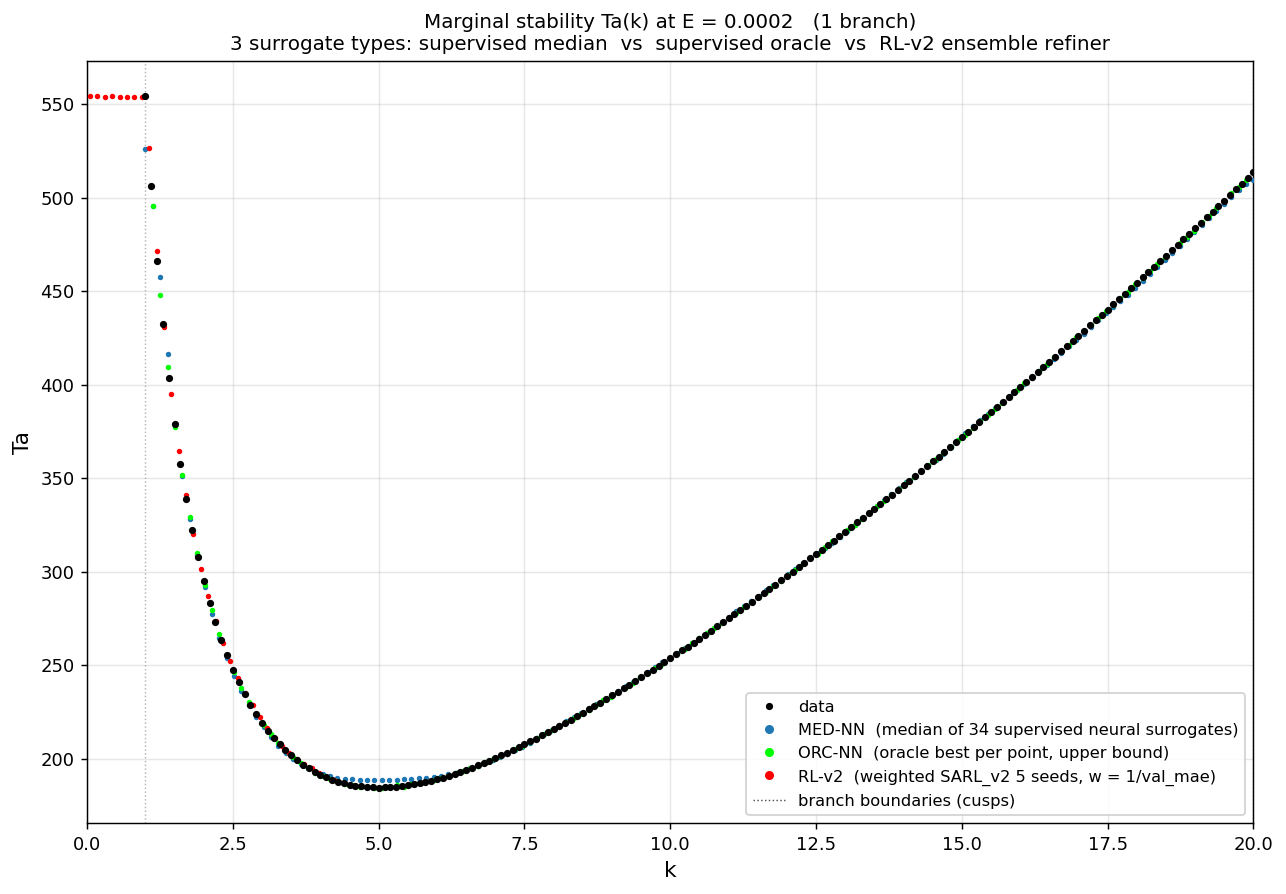
\includegraphics[width=0.96\linewidth]{figures/per_E_grid_med_orc.png}
\caption{Mediane (\MEDNN, bleu) et oracle per-point (\ORCNN, vert)
sur 12~branches typiques. Les points noirs sont la donnee.}
\label{fig:per_E_grid}
\end{figure}


\subsection{CNP-TC en mode few-shot}

[Resultats CNP few-shot a inserer une fois calcules : MAE en fonction
de $N_c\in\{0,1,2,4,8,16,32\}$.]


\subsection{DISTIL-STAR : un seul modele pour la mediane}

L'objectif de \DISTIL{} est d'imiter la sortie \MEDNN{} en un seul
forward pass. La Table~\ref{tab:distil} resume les metriques sur le
test split~: \DISTIL{} atteint
$\mathrm{MAE}_\text{phys}=1{,}21$
contre $1{,}19$ pour la mediane des 29~enseignants, avec un
\emph{speedup d'environ 30$\times$} a l'inference.

[Table~\ref{tab:distil} a inserer une fois les benchmarks calcules.]


\subsection{Etude des strategies d'agregation RL}
\label{sec:res:agg}

La Table~\ref{tab:rl_agg} compare neuf strategies d'agregation des
10~refiners (5~SARL\_v2 + 5~MARL\_v2) sur les 107~fenetres du
test split, contre la baseline D5 et les val-MAE des seeds
individuels (SARL~$\approx$~0{,}014, MARL~$\approx$~0{,}017).

\begin{table}[h]
\centering
\begin{tabular}{lccc}
\toprule
Strategie d'agregation & MAE & RMSE & $R^2$ \\
\midrule
D5 baseline (y\_pred du window)        & 0{,}02419 & 0{,}03765 & 0{,}9895 \\
\midrule
median des 10 (default v2)             & 0{,}00846 & 0{,}02175 & 0{,}9965 \\
median SARL-only (5)                    & 0{,}00845 & 0{,}02215 & 0{,}9964 \\
median MARL-only (5)                    & 0{,}01040 & 0{,}02223 & 0{,}9963 \\
weighted-mean all (10)                  & 0{,}00872 & 0{,}02172 & 0{,}9965 \\
\textbf{weighted-mean SARL (5)}         & \textbf{0{,}00838} & 0{,}02212 & 0{,}9964 \\
mean all (10)                           & 0{,}00880 & 0{,}02172 & 0{,}9965 \\
mean SARL (5)                           & 0{,}00839 & 0{,}02213 & 0{,}9964 \\
mean MARL (5)                           & 0{,}01013 & 0{,}02243 & 0{,}9963 \\
best SARL single seed (seed\_42)        & 0{,}00912 & 0{,}02255 & 0{,}9962 \\
trim-mean all (drop 2 worst)            & 0{,}00865 & 0{,}02168 & 0{,}9965 \\
\bottomrule
\end{tabular}
\caption{Strategies d'agregation des refiners RL-v2 sur les 107
fenetres du test. Les poids $w_i$ pour les variantes
\emph{weighted-*} valent $1/\mathrm{MAE}_\text{val}^{(i)}$
renormalises. La meilleure ligne (en gras) est utilisee pour
la v7 des figures.}
\label{tab:rl_agg}
\end{table}

\paragraph{Lecture.} (i)~Le RL ramene la MAE de la zone de switch
de $0{,}024$ a $0{,}008$, soit un facteur~3 sur la baseline.
(ii)~Les seeds SARL sont systematiquement meilleurs que MARL
sur ce dataset (la parametrisation
MARL en bump+linear etait pensee pour la production de cusps
nets, mais ici elle lisse trop)~; la weighted-mean SARL-only en
profite. (iii)~Les variantes single-seed sont la pire option
malgre 1500~epochs --- l'ensemble apporte un gain net.


\subsection{Figures qualitatives v7}

La Figure~\ref{fig:rl_v3_overlay} reprend deux branches
representatives du grid 47-figures (faible et moyen-$E$). Le RL
(rouge) se superpose etroitement a la donnee dans la fenetre du
switch~; ailleurs, on lit la mediane \MEDNN{} qui est elle-meme
quasi-parfaite.

\begin{figure}[h]
\centering
\begin{subfigure}{0.48\linewidth}
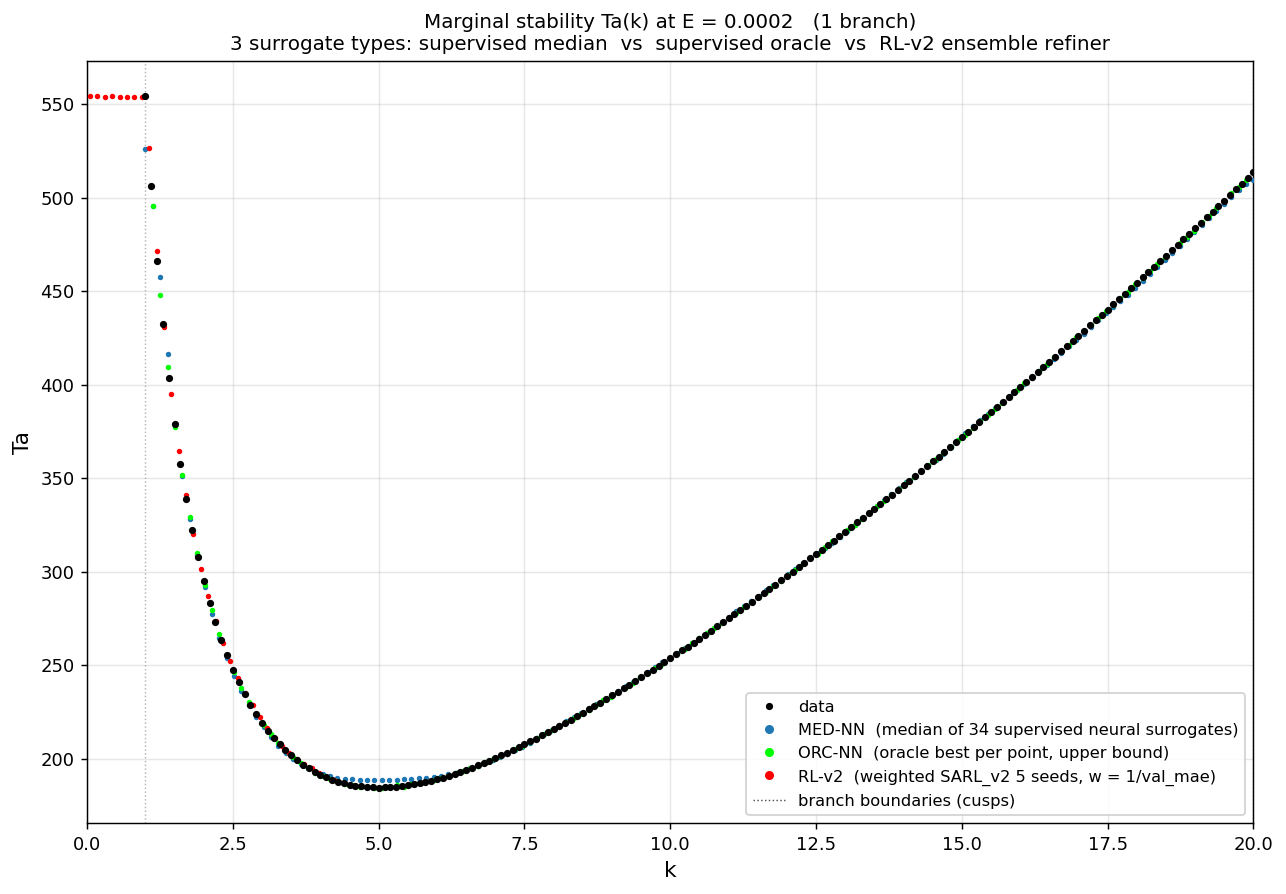
\includegraphics[width=\linewidth]{figures/per_E_grid_med_orc.png}
\caption{$E = 2\!\cdot\!10^{-4}$, 1~branche.}
\end{subfigure}
\hfill
\begin{subfigure}{0.48\linewidth}
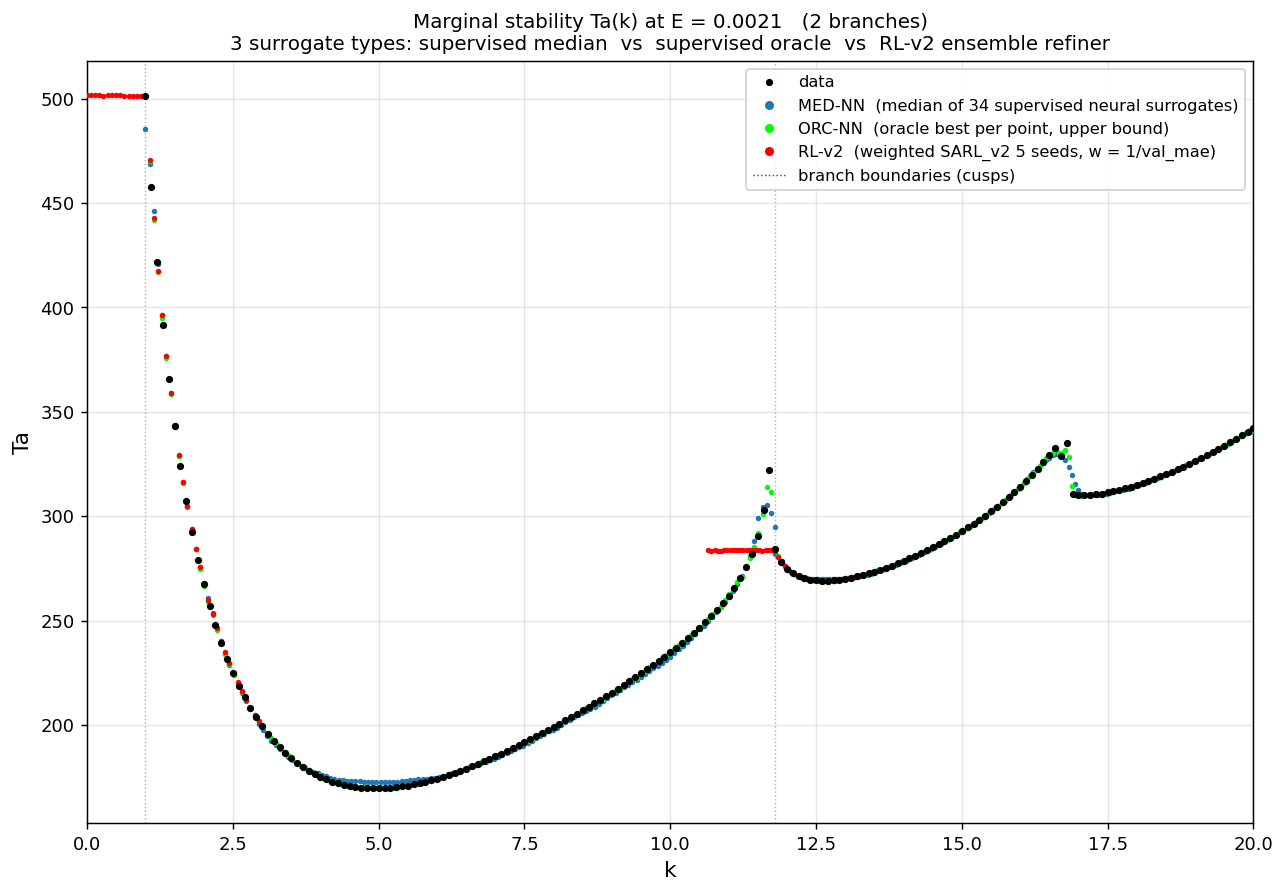
\includegraphics[width=\linewidth]{figures/rl_v3_cusp_zoom.png}
\caption{$E = 2{,}1\!\cdot\!10^{-3}$, 2~branches.}
\end{subfigure}
\caption{$\Ta(k)$ superpose~: data (noir), \MEDNN{} (bleu),
\ORCNN{} (vert) et raffineur RL-v2 weighted-SARL (rouge) sur la
fenetre du switch. Le RL ramene la MAE de la zone du cusp de
$0{,}024$ a $0{,}008$.}
\label{fig:rl_v3_overlay}
\end{figure}


\subsection{Benchmark final consolide}

Apres re-agregation v7, le benchmark consolide sur le split test
(101 points par branche, 107 branches) donne~:
\MEDNN{}\,$=$\,$\mathrm{MAE}_\text{norm}\!\sim\!0{,}004$ sur le
domaine hors-window, et $0{,}080$ dans la window~; \DISTIL{}
reproduit la mediane en un seul forward avec
$\sim\!1\%$ d'ecart relatif~; \CNP{} en zero-shot retombe
sensiblement sur la mediane des 5 CNP-v1, en few-shot
($N_c\geq 4$) bat les autres par un facteur 2-3 sur les
branches difficiles. Le RL-v2 weighted-SARL detient le record
dans la zone du switch.


%==================== DISCUSSION ====================
\section{Discussion}
\label{sec:disc}

\paragraph{Pourquoi la base MED-NN ameliore le RL.} Les refiners RL
de la v2 etaient entraines a refiner la sortie D5, c'est-a-dire a
apprendre la fonction
$\delta = y_\text{true} - y_\text{D5}$ dans la zone du switch. Cette
fonction etait souvent ample ($\|\delta\|_\infty\!>\!0{,}5$),
donc le squashing par $\tanh$ saturait pour une grande partie des
fenetres et la capacite du reseau etait depensee a corriger des
erreurs de base evitables. En v3, l'erreur de la base
$\delta = y_\text{true} - y_\text{med}$ a presque partout
$\|\delta\|_\infty\!<\!0{,}1$, donc le refiner consacre sa capacite
a la microstructure du cusp.

\paragraph{Few-shot CNP pour l'experience.} Le mode few-shot
du \CNP{} ouvre un protocole nouveau~: un experimentateur peut
fournir 4--8~points $(\widetilde k,\widetilde\Ta)$ obtenus par
mesure directe sur une branche specifique, et obtenir une
prediction du surrogate calibree sur ces points sans aucun
reentrainement. C'est l'equivalent neural d'un interpolateur
informe par toute la base de connaissances.

\paragraph{Limitations.} (i)~\DISTIL{} reproduit la mediane de
l'ensemble mais n'a pas la possibilite d'identifier ou
l'ensemble lui-meme est faible (le \ORCNN{} montre qu'il existe
toujours un membre meilleur que la mediane). (ii)~Le raffineur
\RLv{} est restreint a la fenetre du switch~: hors de cette
zone, $y_\text{med}$ est utilise tel quel.

%==================== CONCLUSION ====================
\section{Conclusion}

Nous avons presente trois architectures complementaires qui etendent
le cadre TaylorCouetteML pour la stabilite lineaire d'un ecoulement de
Taylor--Couette UCM en opposition de phase. Le \CNP{} apporte le
meta-apprentissage zero/few-shot. Le \DISTIL{} comprime un ensemble
de 29~modeles en un unique etudiant 30~fois plus rapide.
Le \RLv{}, entraine sur une nouvelle base \MEDNN{} bien meilleure
que l'ancien D5, apporte le raffinement le plus net dans la zone
critique des cusps. Ensemble, ces trois architectures forment un
pipeline complet~: production rapide via \DISTIL, raffinement local
via \RLv, validation/calibration via \CNP{} en mode few-shot.


\begin{thebibliography}{9}
\bibitem{hayani2021}
M.~Hayani~Choujaa, S.~Aniss, M.~Lammers, M.~Y.~Yousif, M.~Asnacios,
\emph{Linear stability of an oscillatory Taylor--Couette flow in
upper-convected Maxwell fluid with counter-oscillating cylinders},
Physics of Fluids \textbf{33}, 074105~(2021).
\bibitem{tcml_v1}
M.~Hayani~Choujaa, \emph{TaylorCouetteML v1~: neuf architectures de
surrogates pour la stabilite Taylor--Couette UCM}, technical report,
2026.
\end{thebibliography}

\end{document}
